        \clearpage
        \begin{figure*}[ht]
            \pdfbookmark[2]{ID 01}{figure_id_01}
        	\centering
            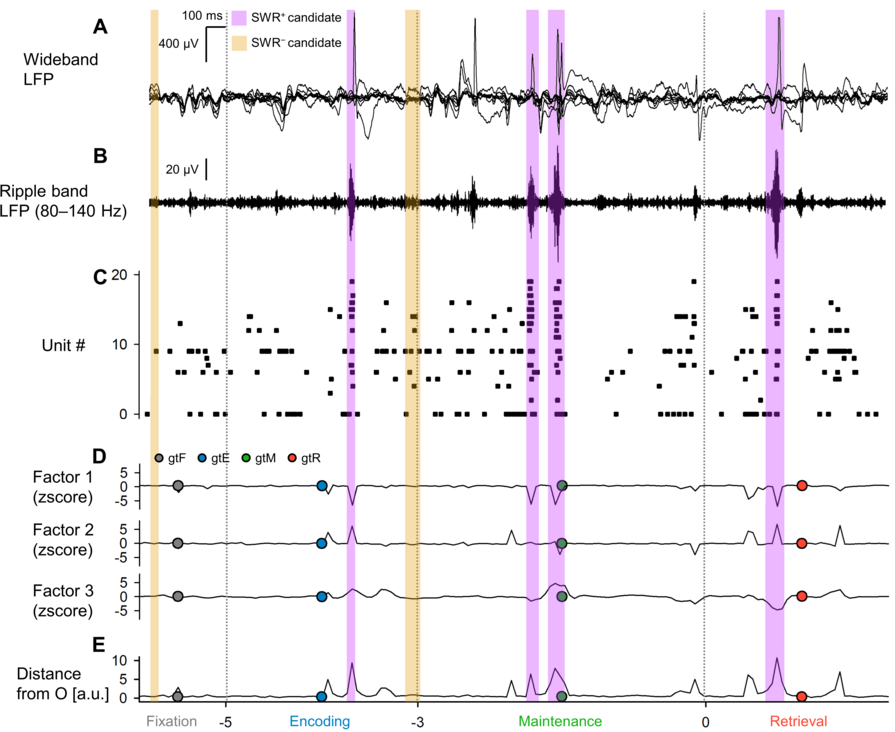
\includegraphics[width=1\textwidth]{./src/figures/.png/Figure_ID_01.png}
        	\caption{\textbf{Local field potential (LFP), multiunit activity, and neural trajectory of the hippocampus during a modified Sternberg task} \cite{li_functional_2023, borders_hippocampal_2022, dimakopoulos_information_2022}}
\smallskip
\\
\textbf{\textit{A.}} Representative wideband LFP traces from iEEG signals recorded in the left hippocampal head. These were attained while the subject performed a modified Sternberg working memory task, consisting of fixation (1 s, \textit{gray}), encoding (2 s, \textit{blue}), maintenance (3 s, \textit{green}), and retrieval (2 s, \textit{red}) \cite{li_functional_2023, borders_hippocampal_2022, dimakopoulos_information_2022}. \textbf{\textit{B.}} The corresponding ripple band LFP traces \cite{schomburg_spiking_2012, behrens_induction_2005, norimoto_hippocampal_2018}. \textbf{\textit{C.}} The raster plot of multiunit spikes derived from the LFP traces using a spike sorting algorithm \cite{niediek_reliable_2016}. \textbf{\textit{D.}} Neural trajectory determined by GPFA on the basis of spike counts per unit with 50-ms bins \cite{yu_gaussian-process_2009}. The dot circles represent the geometric median coordinates for each phase. \textbf{\textit{E.}} Trajectory distance from the origin $O$. Please note that the \textit{purple} and \textit{yellow} rectangles indicate the timings for SWR$^+$ candidates and SWR$^-$ candidates (controls for SWR$^+$), respectively \cite{van_vugt_hippocampal_2010, scoville_loss_1957, kay_hippocampal_2016, nader_memory_2003, wilson_reactivation_1994, nadasdy_replay_1999, lee_memory_2002}.
}
% width=1\textwidth
        	\label{fig:01}
        \end{figure*}
